% Number 290
% CVPMA Algebra Units
% Avg. v, speed, dsiplacement
% JG

% Watermark
\AddToShipoutPicture*{\BackgroundPic}

\addtocounter {ProbNum} {1}

%\begin{floatingfigure}[r]{.3\textwidth}
%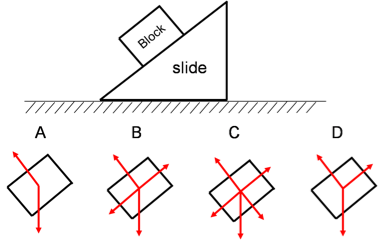
\includegraphics[scale=.4]{/Users/jgates/desktop/latex/pics/incline3.png}
%\end{floatingfigure}
 
{\bf \Large{\arabic{ProbNum}}}A squirrel runs back and forth on a fence rail.  It runs east 4 meters in 1.2 seconds, then pauses for .8 seconds, then runs west 6 meters in 1.3 seconds, and then east 7 meters in 4 seconds.

\bigskip
What was the squirrel's maximum speed?

\vfill
What was the squirrel's average speed during the trip?

\vfill
What was the squirrel's average velocity during the trip (give a complete answer to this question!)?

\vfill
What was the squirrel's displacement during the first 3 seconds?
 
%\begin{center}
%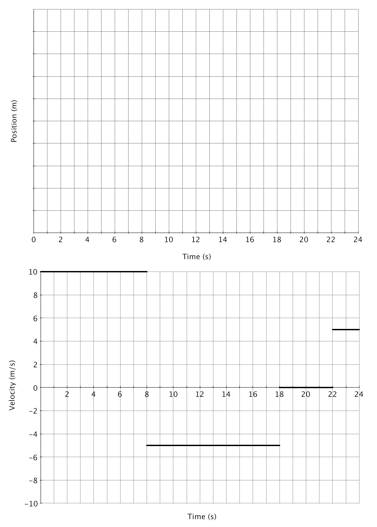
\includegraphics[scale=.77]{/Users/jgates/desktop/latex/pics/vtoxgraph1.png}
%\end{center}
 
\vfill

\newpage